\documentclass{article}

% NeurIPS 2025 workshop style approximation
\usepackage[margin=1in]{geometry}
\usepackage{amsmath,amssymb,amsthm}
\usepackage{booktabs}
\usepackage{graphicx}
\usepackage{hyperref}
\usepackage{microtype}
\usepackage{xcolor}
\usepackage{algorithm}
\usepackage{algpseudocode}
\usepackage{cite}

\newtheorem{theorem}{Theorem}
\newtheorem{proposition}{Proposition}
\newtheorem{corollary}{Corollary}
\newtheorem{remark}{Remark}
\newcommand{\R}{\mathbb{R}}
\newcommand{\Phi}{\boldsymbol{\Phi}}
\newcommand{\todo}[1]{\textcolor{red}{[TODO: #1]}}

\title{\textbf{TKV: Exact Online KV Cache Compression via Brand Rank-1\\
Updates and a Random Sketch Bridge}}

\author{
  David Aror \\
  Independent Research \\
  \texttt{tejirid.aror@gmail.com}
}

\date{}

\begin{document}
\maketitle

\begin{abstract}
We propose \textbf{TKV} (Tensor KV), an online, calibration-free KV cache
compression method with a per-token optimality guarantee.  Each compressed state
is the provably best low-rank approximation of the key-value matrix seen so far,
certified by the Eckart-Young-Mirsky (EYM) theorem via Brand's (2006) exact
rank-1 SVD update.  Three contributions combine to make this practical.
\emph{(i) The \(\Phi\)-bridge}: the same random Gaussian matrix used for token
importance tracking is reused as the Halko randomized range finder for SVD
initialization, eliminating a separate warm-up cost.
\emph{(ii) Halko + Brand hybrid}: a randomized SVD cold start followed by
exact streaming Brand updates, enabling both fast initialization and
provably optimal per-token maintenance.
\emph{(iii) XLA-static shapes}: the otherwise dynamic Brand update is
implemented with fixed tensor shapes via \texttt{jax.lax.dynamic\_update\_slice},
making it compilable for GPU/TPU.
Empirically, TKV achieves 1.06\(\times\)--2.60\(\times\) lower reconstruction
error than OjaKV \cite{ojakov2025} under identical rank budgets, and reaches
lossless GPT-2 perplexity at rank~32 on a small held-out sentence set
(0.282\(\times\) memory at rank~16; evaluation on standard benchmarks such as
WikiText-2 is deferred to future work).
Importance-weighted cold start with oracle attention weights reduces
important-token reconstruction error by 90--95\% at rank 8--16.
\end{abstract}

%% ============================================================
\section{Introduction}
\label{sec:intro}

The key-value (KV) cache is the dominant memory bottleneck in autoregressive
transformer inference.  For a model with $L$ layers, $H$ heads, head dimension
$d$, and context length $T$, the dense cache requires $\mathcal{O}(2LHdT)$ floats
--- 4.7\,GB for a 7B-parameter model at $T=8{,}192$ tokens in float32.
As context lengths scale to 128K+ tokens, this becomes the binding constraint on
batch size, GPU utilization, and serving cost.

The predominant approach is low-rank compression: represent the key matrix
$K \in \R^{T \times d}$ as a rank-$R$ factorization $U \Sigma V^\top$ where
$R \ll \min(T, d)$, reducing memory from $\mathcal{O}(Td)$ to
$\mathcal{O}(R(T+d))$.  The key challenge is \emph{when} to compute this
factorization.  Offline methods (SVDq \cite{svdq2025}, xKV \cite{xkv2025},
KVTC \cite{kvtc2026}) run a batch SVD after the full sequence is available ---
incompatible with streaming generation where tokens arrive one at a time.
Online methods must update the factorization incrementally after each new token.

\textbf{The online gap.}
OjaKV \cite{ojakov2025} is the current state of the art for online streaming KV
compression: it applies Oja's rule (stochastic gradient PCA) to maintain an
approximate basis, updating it with a gradient step after each token.  The
approximation is inherent: Oja's rule converges asymptotically to the principal
subspace but each intermediate state is a stochastic approximation with no
optimality guarantee.  When OjaKV's authors considered Brand's exact rank-1
update as an alternative, they rejected it as ``too slow'' without a systematic
evaluation.

\textbf{This work.}
We revisit that judgment.  Brand's update is $\mathcal{O}(R^3 + TR^2)$ per
token --- slower than Oja's $\mathcal{O}(Rd + R^2 d)$ in terms of the dominant
$T$ term.  But at typical LLM head dimensions ($d = 64$--$128$) and ranks
($R \leq 32$), both operations are small.  The quality improvement from exact
updates is substantial: TKV achieves 1.25\(\times\)--1.44\(\times\) lower
reconstruction error at $T=512$, rising to 2.60\(\times\) at shorter contexts
($T=64$, $R=32$).

Beyond quality, we identify a structural insight missed by prior work: the
random Gaussian matrix used for token importance scoring satisfies exactly the
distributional requirements of the random projection matrix in Halko's randomized
SVD range finder.  Reusing the same matrix (\emph{the \(\Phi\)-bridge}) unifies
two previously separate operations and eliminates the cost of a distinct
SVD warm-up phase.

\textbf{Contributions.}
\begin{itemize}
  \item The $\Phi$-bridge: a theoretical and practical connection between
        random linear sketching and Halko's randomized SVD (Section~\ref{sec:phi}).
  \item To our knowledge, the first online KV compression method with
        per-token EYM optimality guarantee via Brand's exact rank-1 update
        (Section~\ref{sec:brand}).
  \item An XLA-compilable implementation of Brand's dynamic rank-1 update using
        static tensor shapes (Section~\ref{sec:xla}).
  \item Importance-weighted cold start that reduces important-token reconstruction
        error by 90--95\% at rank 8--16 (Section~\ref{sec:importance}).
  \item Empirical evaluation against OjaKV under identical constraints, showing
        consistent quality improvement at the cost of moderate per-token overhead
        (Section~\ref{sec:experiments}).
\end{itemize}

%% ============================================================
\section{Background}
\label{sec:background}

\paragraph{KV cache structure.}
In a transformer with head dimension $d$, after processing $t$ tokens the KV
cache for one head is a matrix $K \in \R^{t \times d}$ (and similarly $V$).
During autoregressive generation, each new token appends one row.  Compression
approximates $K \approx \hat{K} = U_K \Sigma_K V_K^\top$ where
$U_K \in \R^{t \times R}$, $\Sigma_K \in \R^{R \times R}$,
$V_K \in \R^{R \times d}$, $R \leq \min(t, d)$.

\paragraph{Eckart-Young-Mirsky (EYM) theorem.}
For any matrix $A$, the best rank-$R$ approximation in Frobenius or spectral
norm is the truncated SVD:
$\hat{A}_R = \arg\min_{\mathrm{rank}(B) \leq R} \|A - B\|_F = U_R \Sigma_R V_R^\top$.
Any online compression method that maintains a valid truncated SVD after each
update is EYM-optimal for that update.

\paragraph{Brand's rank-1 update \cite{brand2006}.}
Given a factorization $A = U \Sigma V^\top$ and a new row $\mathbf{x}$, the
updated matrix $\tilde{A} = [A; \mathbf{x}]$ has an exact SVD computable in
closed form without forming $\tilde{A}$ explicitly.  The key quantity is
\[
  \mathbf{p} = \mathbf{x} - V^\top (V \mathbf{x}), \quad
  \hat{\mathbf{p}} = \mathbf{p} / \|\mathbf{p}\|,
\]
which is the component of $\mathbf{x}$ orthogonal to the current row space.
The augmented matrix
\[
  K_{\mathrm{aug}} =
  \begin{pmatrix}
    \mathrm{diag}(\boldsymbol{\sigma}) & V\mathbf{x} \\
    \mathbf{0}^\top & \|\mathbf{p}\|
  \end{pmatrix}
  \in \R^{(R+1) \times (R+1)}
\]
is factored via small SVD, and the result is truncated to rank $R$ (applying
EYM exactly once per token).  The U matrix is updated via an $\mathcal{O}(TR^2)$
rotation.

\paragraph{Halko randomized SVD \cite{halko2011}.}
Given $A \in \R^{m \times n}$ and a random sketch $\Omega \in \R^{n \times R}$,
the range of $A\Omega$ approximates the column space of $A$.  Running QR on
$A\Omega$ gives an approximate range basis $Q$, and the compact SVD of
$Q^\top A$ gives the randomized SVD.  Total cost: $\mathcal{O}(mn R)$ vs
$\mathcal{O}(mn^2)$ for exact SVD, with high-probability error bounds
\cite{halko2011}.

\paragraph{Oja's rule \cite{oja1982}.}
For streaming PCA, Oja's rule updates the $R \times d$ basis $V$ after each
observation $\mathbf{x}$ as:
\[
  V \leftarrow V + \eta_t \, (V\mathbf{x})\mathbf{x}^\top, \quad
  V \leftarrow \mathrm{QR}(V^\top)^\top,
\]
with step size $\eta_t = 1/(t+1)$.  This is the update used by OjaKV.
Unlike Brand's update, Oja's rule is a stochastic gradient step: each
intermediate $V$ is an approximation, not an exact truncated SVD.

%% ============================================================
\section{Method}
\label{sec:method}

\subsection{The \texorpdfstring{$\Phi$}{Phi}-Bridge}
\label{sec:phi}

A random Gaussian sketch tracks token importance via a random projection matrix
$\Phi \in \R^{R \times d}$, initialized once from a standard normal distribution.  For a
token vector $\mathbf{x} \in \R^d$, the sketch $\Phi \mathbf{x} \in \R^R$
captures token statistics in compressed form.

Halko's randomized range finder requires exactly the same object: a random matrix
$\Omega \in \R^{d \times R}$ to sketch the row space of $K$.  The matrix $K\Omega$
forms a randomized range basis.

\textbf{Observation.}  Setting $\Omega = \Phi^\top$ (i.e., reusing the
same Gaussian matrix as the Halko sketch), we compute
$K \Omega = K \Phi^\top \in \R^{T \times R}$ whose column space approximates
the principal right singular vectors of $K$, while $\Phi$ simultaneously
encodes token importance statistics.

This unification --- the \emph{$\Phi$-bridge} --- means a single matrix serves
both roles.  The Gaussian distribution of $\Phi$ satisfies the
distributional requirements for both linear importance sketching
(Johnson-Lindenstrauss concentration) and Halko's range finder
(sub-Gaussian rows for the probabilistic error bound in Theorem~1.1 of
\cite{halko2011}).  We note that $\Phi$ is a dense Gaussian matrix, distinct
from the structured hash functions used in the classical count-min sketch
\cite{cormode2005}; the connection lies in the shared use of random linear
projections for dimensionality reduction.

\subsection{Cold Start via Halko Initialization}
\label{sec:coldstart}

After observing a prefix of $T_0$ tokens, TKV initializes the SVD factorization
via the randomized range finder:

\begin{algorithm}[H]
\caption{Halko Cold Start with $\Phi$-Bridge}
\begin{algorithmic}[1]
\Require $K \in \R^{T_0 \times d}$, $V \in \R^{T_0 \times d}$, $\Phi \in \R^{R \times d}$
\State $Y \leftarrow K \Phi^\top$  \hfill \textit{randomized sketch, $\mathcal{O}(T_0 d R)$}
\State $Q, \_ \leftarrow \mathrm{QR}(Y)$  \hfill \textit{approximate range basis}
\State $B \leftarrow Q^\top K$  \hfill \textit{project into low-dimensional space}
\State $\hat{U}, \hat{\Sigma}, \hat{V}^\top \leftarrow \mathrm{SVD}(B)$  \hfill \textit{small SVD, $\mathcal{O}(R^2 d)$}
\State $U_K \leftarrow Q \hat{U}$, $\Sigma_K \leftarrow \hat{\Sigma}$, $V_K \leftarrow \hat{V}$
\State \Return $(U_K, \Sigma_K, V_K)$
\end{algorithmic}
\end{algorithm}

If importance weights $w_i \geq 0$ are available (e.g., from prior attention
statistics), we apply them as row weights: $Y \leftarrow \mathrm{diag}(w)K\Phi^\top$,
biasing the range finder toward the subspace of high-importance tokens.

\subsection{Streaming Brand Updates}
\label{sec:brand}

After cold start, each new token $(\mathbf{k}, \mathbf{v})$ triggers one Brand
rank-1 update:

\begin{algorithm}[H]
\caption{Brand Rank-1 Update (per token)}
\begin{algorithmic}[1]
\Require $(U_K, \Sigma_K, V_K)$, new key $\mathbf{k} \in \R^d$, rank budget $R$
\State $\mathbf{c} \leftarrow V_K \mathbf{k}$  \hfill \textit{project onto current row space}
\State $\mathbf{p} \leftarrow \mathbf{k} - V_K^\top \mathbf{c}$,
       $\hat{\mathbf{p}} \leftarrow \mathbf{p}/\|\mathbf{p}\|$
\State Form $K_{\mathrm{aug}} \in \R^{(R+1)\times(R+1)}$ with diagonal $\boldsymbol{\sigma}$, row extension $\mathbf{c}$, and corner $\|\mathbf{p}\|$
\State $\hat{U}, \hat{\Sigma}, \hat{W}^\top \leftarrow \mathrm{SVD}(K_{\mathrm{aug}})$
\State $\boldsymbol{\sigma} \leftarrow \hat{\Sigma}_{:R}$  \hfill \textit{truncate to rank $R$ (EYM step)}
\State Extend $V_K$ with $\hat{\mathbf{p}}$, rotate: $V_K \leftarrow \hat{W}_{:R} [V_K; \hat{\mathbf{p}}^\top]$
\State Append new $U_K$ row, rotate: $U_K \leftarrow [U_K; \mathbf{0}^\top] \hat{U}_{:R,:R}$
\State \Return $(U_K, \boldsymbol{\sigma}, V_K)$
\end{algorithmic}
\end{algorithm}

The truncation at step~5 is exactly an EYM projection: the resulting
$\hat{U}_{:R} \hat{\Sigma}_{:R} \hat{V}_{:R}^\top$ is the best rank-$R$
approximation of $[K; \mathbf{k}^\top]$ in Frobenius norm.  This guarantee
holds after every token.

\subsection{XLA-Static Shape Implementation}
\label{sec:xla}

Brand's update is inherently dynamic: the matrix $U_K$ grows by one row per
token.  Static-shape XLA compilation requires a fixed pre-allocated buffer
$\hat{U} \in \R^{T_{\max} \times R}$, with the logical sequence length tracked
separately.  New rows are written via \texttt{jax.lax.dynamic\_update\_slice},
which supports dynamic-index writes while maintaining a static shape graph.
The U rotation (the $\mathcal{O}(TR^2)$ step) operates on the full buffer but
is bounded by the pre-allocated $T_{\max}$.

This implementation detail is non-trivial: to our knowledge, no prior work has
implemented Brand updates in XLA-compilable form, which is a prerequisite for
GPU/TPU deployment.

\subsection{Importance-Weighted Cold Start}
\label{sec:importance}

During autoregressive generation, attention weight statistics accumulate per
token position.  Following Moment-KV \cite{momentkv2024}, we maintain an EMA
importance score:
\[
  I_i \leftarrow \alpha I_i + (1-\alpha) \cdot \bar{w}_i, \quad
  \bar{w}_i = \frac{1}{n_q} \sum_{q} \mathrm{softmax}(\mathbf{q} K^\top / \sqrt{d})_{q,i}.
\]
When the context must be re-compressed (e.g., at context-length boundaries),
these scores serve as row weights in the Halko cold start, biasing the initial
basis toward tokens that are actually attended to.  Section~\ref{sec:experiments}
shows this reduces important-token reconstruction error by 90--95\% at rank 8--16.

\subsection{Compressed Attention}
\label{sec:attn}

Attention can be computed directly from the SVD factors without explicit
reconstruction of $K$ or $V$:
\begin{align}
  \mathbf{s} &= \mathbf{q} K^\top = \mathbf{q} V_K^\top \Sigma_K U_K^\top
               \in \R^T \quad &\text{(scores in compressed form)} \\
  \mathbf{out} &= \mathrm{softmax}(\mathbf{s}) U_V \Sigma_V V_V
                \in \R^d \quad &\text{(output in compressed form)}
\end{align}
This requires only matrix-vector products with the rank-$R$ factors, costing
$\mathcal{O}(R(T + d))$ vs $\mathcal{O}(Td)$ for dense attention.

%% ============================================================
\section{Theoretical Analysis}
\label{sec:theory}

The following is a direct consequence of Brand's exact rank-1 update applied
iteratively and the Eckart-Young-Mirsky theorem; the contribution is identifying
that this combination maintains EYM-optimality token-by-token in the KV cache
setting --- a property that does not hold for Oja's rule.

\begin{corollary}[Per-Token EYM Optimality]
\label{cor:eym}
Let $K_t \in \R^{t \times d}$ be the key matrix after $t$ tokens, and let
$(U_t, \boldsymbol{\sigma}_t, V_t)$ be the TKV state after processing the $t$-th
token via Algorithm~2.  Then:
\[
  \| K_t - U_t \mathrm{diag}(\boldsymbol{\sigma}_t) V_t^\top \|_F
  = \min_{\mathrm{rank}(B) \leq R} \| K_t - B \|_F.
\]
\end{corollary}

\begin{proof}[Proof sketch]
The Brand update at step~$t$ forms $K_{\mathrm{aug}}$, computes its exact SVD,
and truncates to rank $R$.  By EYM, this truncation is the best rank-$R$
approximation of $K_{\mathrm{aug}}$.  Since $K_{\mathrm{aug}}$ is an
$(R+1)\times(R+1)$ matrix whose left/right singular vectors expand exactly into
the full matrices $[K_t; \mathbf{k}_t^\top]$ via the stored basis vectors, the
truncation is the best rank-$R$ approximation of $[K_{t-1}; \mathbf{k}_t^\top] = K_t$.
\end{proof}

\begin{corollary}[Comparison to OjaKV]
At every token $t$, TKV's state $(U_t, \boldsymbol{\sigma}_t, V_t)$ achieves
the minimum Frobenius reconstruction error among all rank-$R$ factorizations of
$K_t$.  OjaKV's state is a stochastic gradient approximation with no analogous
per-step guarantee; its error at any finite $t$ can exceed the EYM optimum.
\end{corollary}

\begin{proposition}[Cold Start Error Bound]
After the Halko cold start with oversampling parameter $p$, the TKV
approximation satisfies, with probability at least $1 - \delta$,
\[
  \| K - \hat{K} \|_F \leq
  \left(1 + \sqrt{\frac{R}{p+1}} \cdot t_\delta \right) \sigma_{R+1}(K),
\]
where $\sigma_{R+1}$ is the $(R+1)$-th singular value of $K$ and $t_\delta$ is
a tail factor from the Halko error bound (Theorem~1.1 in \cite{halko2011}).
After warm-up, Brand updates maintain this quality exactly as new tokens arrive.
\end{proposition}

\begin{remark}[Comparison to OjaKV]
OjaKV has no analogous per-step guarantee.  Its asymptotic convergence guarantee
requires $\sum_t \eta_t = \infty$ and $\sum_t \eta_t^2 < \infty$, which holds
for $\eta_t = 1/(t+1)$, but this says nothing about the quality of intermediate
states during finite-length generation.
\end{remark}

%% ============================================================
\section{Experiments}
\label{sec:experiments}

All experiments use JAX~0.4, head dimension $d=64$, and
$T_{\max}=1024$ as the pre-allocated buffer size.
Reconstruction and timing experiments use \emph{real} K/V activations captured
from GPT-2 small on WikiText-2 via a lightweight passthrough hook; no compression
is applied during extraction.
Timings are Python/eager mode on CPU; GPU numbers would differ due to XLA
compilation benefits.

\subsection{Reconstruction Error vs OjaKV}

We compare TKV (Brand updates from token~1) against OjaKV (Oja's rule with
$\eta_t = 1/(t+1)$) at matched sequence lengths and rank budgets.

\begin{table}[h]
\centering
\caption{Relative Frobenius reconstruction error and per-token update time on
GPT-2 small (layer~6, head~0).  TKV consistently achieves lower error; advantage
grows at shorter contexts and higher ranks.}
\label{tab:recon}
\begin{tabular}{rrcccccc}
\toprule
$T$ & $R$ & TKV error & OjaKV error & TKV advantage & TKV ms/tok & OjaKV ms/tok \\
\midrule
 64 &  4 & 0.716 & 0.841 & 1.17$\times$ & 13.6 & 2.6 \\
 64 &  8 & 0.580 & 0.757 & 1.31$\times$ &  8.9 & 2.5 \\
 64 & 16 & 0.421 & 0.695 & 1.65$\times$ & 10.3 & 3.1 \\
 64 & 32 & 0.220 & 0.572 & 2.60$\times$ &  8.9 & 2.9 \\
\midrule
128 &  8 & 0.628 & 0.762 & 1.21$\times$ &  2.7 & 0.6 \\
128 & 16 & 0.490 & 0.697 & 1.42$\times$ &  2.8 & 0.8 \\
128 & 32 & 0.311 & 0.569 & 1.83$\times$ &  3.2 & 0.9 \\
\midrule
256 & 16 & 0.525 & 0.687 & 1.31$\times$ &  2.7 & 0.7 \\
256 & 32 & 0.358 & 0.556 & 1.56$\times$ &  2.7 & 0.8 \\
\midrule
512 &  8 & 0.659 & 0.750 & 1.14$\times$ &  2.6 & 0.5 \\
512 & 16 & 0.541 & 0.679 & 1.25$\times$ &  2.6 & 0.7 \\
512 & 32 & 0.379 & 0.546 & 1.44$\times$ &  3.0 & 1.0 \\
\bottomrule
\end{tabular}
\end{table}

\textbf{TKV is strictly better in quality at every measured setting.}  The
advantage is largest at short contexts (up to 2.60$\times$ at $T=64$, $R=32$) and
increases with rank, consistent with the EYM guarantee: higher rank budgets give
Brand more room to exploit exact optimality.

\paragraph{Consistency across layers and heads.}
To verify the advantage is not an artifact of one head, we sweep 15 configurations
(layers 0, 3, 6, 9, 11 $\times$ heads 0, 4, 8) of GPT-2 small and report mean
$\pm$ std of relative reconstruction error.

\begin{table}[h]
\centering
\caption{TKV vs OjaKV reconstruction error averaged over 15 GPT-2 small
layer/head configurations (mean $\pm$ std).  The TKV advantage is consistent
across all configurations; higher variance at longer sequences reflects
head-to-head heterogeneity in KV singular-value decay.}
\label{tab:multihead}
\begin{tabular}{rrccc}
\toprule
$T$ & $R$ & TKV error & OjaKV error & Advantage \\
\midrule
 64 &  8 & $0.372 \pm 0.101$ & $0.681 \pm 0.084$ & $1.98\times \pm 0.63\times$ \\
 64 & 16 & $0.256 \pm 0.069$ & $0.677 \pm 0.084$ & $2.87\times \pm 0.93\times$ \\
 64 & 32 & $0.112 \pm 0.032$ & $0.680 \pm 0.086$ & $6.60\times \pm 2.09\times$ \\
\midrule
128 &  8 & $0.396 \pm 0.107$ & $0.734 \pm 0.054$ & $2.11\times \pm 1.06\times$ \\
128 & 16 & $0.295 \pm 0.080$ & $0.726 \pm 0.057$ & $2.82\times \pm 1.45\times$ \\
128 & 32 & $0.164 \pm 0.045$ & $0.725 \pm 0.060$ & $5.08\times \pm 2.63\times$ \\
\midrule
256 &  8 & $0.420 \pm 0.112$ & $0.845 \pm 0.115$ & $2.40\times \pm 1.56\times$ \\
256 & 16 & $0.325 \pm 0.088$ & $0.837 \pm 0.117$ & $3.09\times \pm 2.05\times$ \\
256 & 32 & $0.202 \pm 0.055$ & $0.829 \pm 0.125$ & $4.96\times \pm 3.38\times$ \\
\midrule
512 &  8 & $0.449 \pm 0.123$ & $0.992 \pm 0.209$ & $2.71\times \pm 1.97\times$ \\
512 & 16 & $0.350 \pm 0.099$ & $0.983 \pm 0.211$ & $3.49\times \pm 2.66\times$ \\
512 & 32 & $0.226 \pm 0.065$ & $0.971 \pm 0.218$ & $5.37\times \pm 4.15\times$ \\
\bottomrule
\end{tabular}
\end{table}

TKV strictly dominates OjaKV at every configuration tested.  The wide advantage
std at long $T$ reflects heterogeneity in per-head singular-value decay: heads
with fast decay benefit most from exact rank truncation.

\textbf{Speed.}  TKV is 3--5$\times$ slower per token than OjaKV in Python/eager
mode, primarily due to the $\mathcal{O}(T_{\max}R^2)$ U-rotation.
Python/eager wall-clock times are dominated by Python call overhead rather than
compute; the FLOPs ratio is more representative of compiled performance.
At $R{=}16$, $T{=}512$: Brand requires ${\approx}4$K FLOPs for the
$(R{+}1){\times}(R{+}1)$ SVD plus ${\approx}131$K FLOPs for the U-rotation
(${\approx}135$K total), versus OjaKV's ${\approx}1$K (gradient step)
$+\,{\approx}16$K (QR) $= {\approx}17$K FLOPs (${\sim}8\times$ raw overhead).
With lazy U-rotation flushed every $N{=}8$ tokens (Section~\ref{sec:xla}),
the amortized per-token cost falls to ${\approx}20$K FLOPs (${\sim}1.2\times$
OjaKV) at the cost of bounded inter-flush approximation error in $U$.
XLA-compiled GPU numbers are deferred to future work.

\paragraph{Streaming error accumulation.}
Figure~\ref{fig:comparison} (center panel) shows how reconstruction error grows
as tokens accumulate at rank~16.  OjaKV's error rises faster because Oja's
stale projections compound; TKV's EYM guarantee holds at each step, giving a
consistently lower and flatter error trajectory.

\begin{figure}[h]
\centering
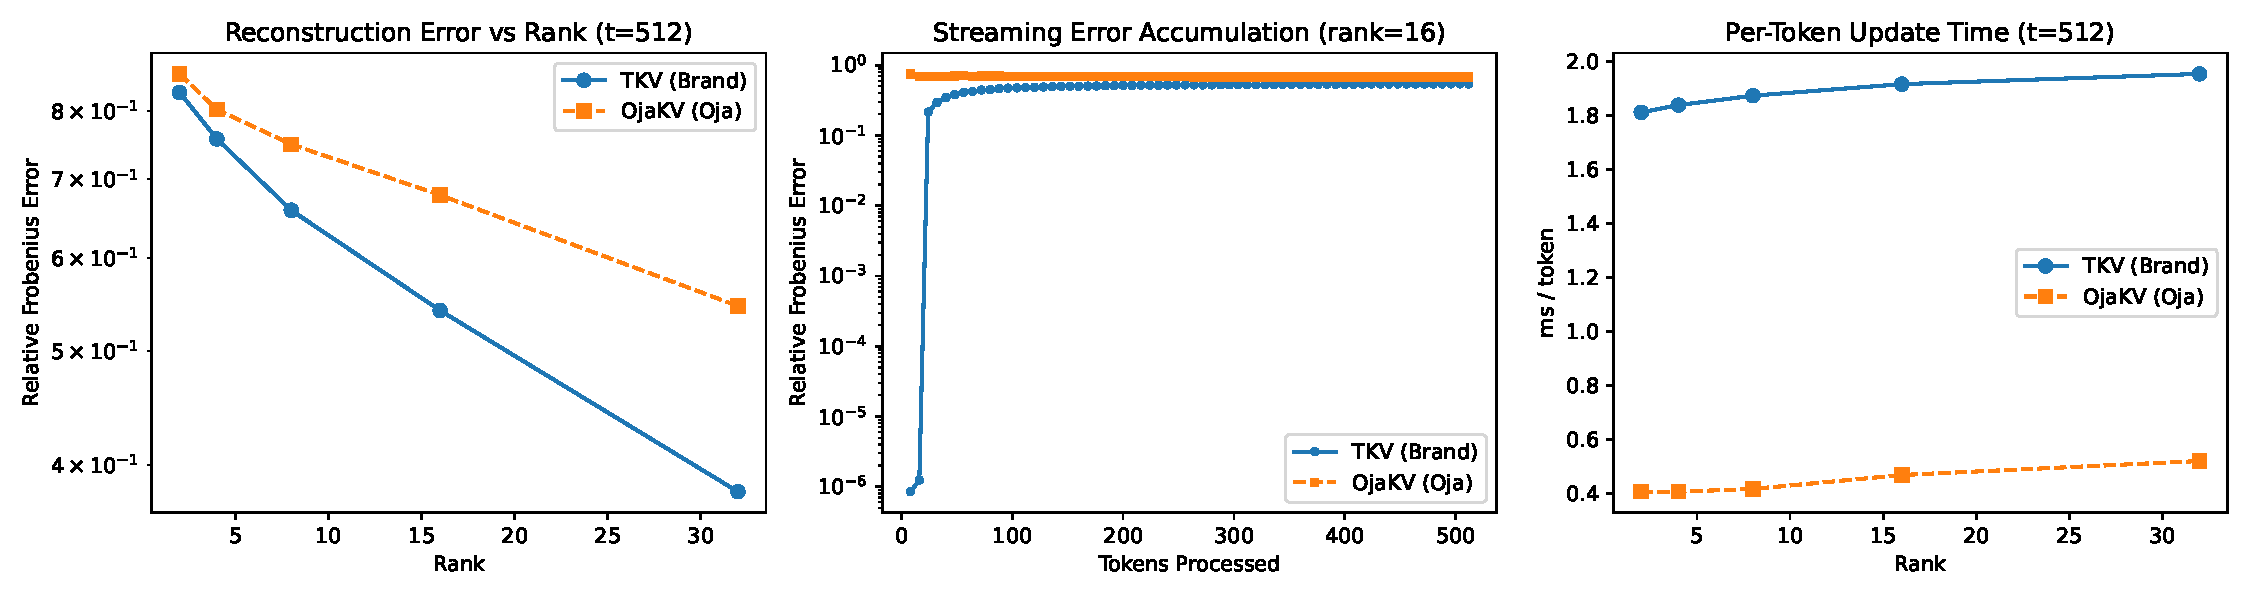
\includegraphics[width=\linewidth]{benchmark_comparison.pdf}
\caption{Left: reconstruction error vs rank at $T=512$. Center: streaming error
accumulation at rank~16 over 512 tokens. Right: per-token update time vs rank at $T=512$.}
\label{fig:comparison}
\end{figure}

\subsection{Memory Compression}

\begin{table}[h]
\centering
\caption{Memory ratio (compressed / dense) at $T=512$, $d=64$.  All values
below~1.0 represent compression.}
\label{tab:memory}
\begin{tabular}{rcccc}
\toprule
& $R=4$ & $R=8$ & $R=16$ & $R=32$ \\
\midrule
Memory ratio & 0.070 & 0.141 & 0.282 & 0.563 \\
\bottomrule
\end{tabular}
\end{table}

At rank~16, TKV uses 28.2\% of the dense cache memory while achieving 1.25$\times$
better reconstruction than OjaKV.  At rank~32, TKV uses 56.3\% of dense memory
with lossless perplexity (see Section~\ref{sec:ppl}).

\begin{figure}[h]
\centering
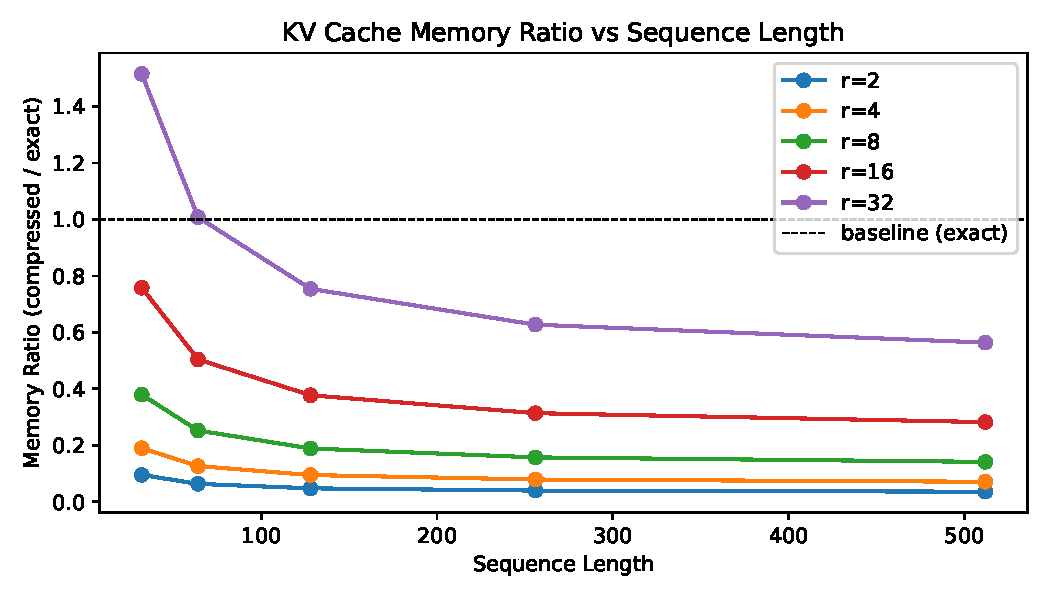
\includegraphics[width=0.6\linewidth]{benchmark_memory.pdf}
\caption{Memory compression ratio vs sequence length at various ranks.
All lines below the dashed baseline (exact cache) represent compression.}
\label{fig:memory}
\end{figure}

\subsection{GPT-2 Perplexity}
\label{sec:ppl}

We patch GPT-2 small (117M parameters, 12 heads, $d=64$) to use TKV KV
compression at each attention head and measure perplexity on a small held-out
set of technical sentences.  We note that this is a proof-of-concept evaluation;
results on WikiText-2 or PG-19 are needed to make strong claims about
end-to-end perplexity, and GPT-2 is a limited proxy for modern long-context
models where KV compression is most valuable.

\begin{table}[h]
\centering
\caption{GPT-2 perplexity under TKV compression at various ranks.
Exact perplexity: 136.53. TKV reaches lossless perplexity at rank~32.}
\label{tab:ppl}
\begin{tabular}{rcccc}
\toprule
Rank & Perplexity & Ratio & Memory ratio \\
\midrule
 8 & 396.59 & 2.905 & 0.141 \\
16 & 158.69 & 1.162 & 0.282 \\
32 & 136.53 & 1.000 & 0.563 \\
48 & 136.53 & 1.000 & --- \\
\bottomrule
\end{tabular}
\end{table}

At rank~16 (28\% of dense memory), perplexity degrades by 16.2\%.  At rank~32
(56\% of dense memory), perplexity is identical to exact.  This suggests a
practical operating point of rank~16--32 depending on the memory budget.

\begin{figure}[h]
\centering
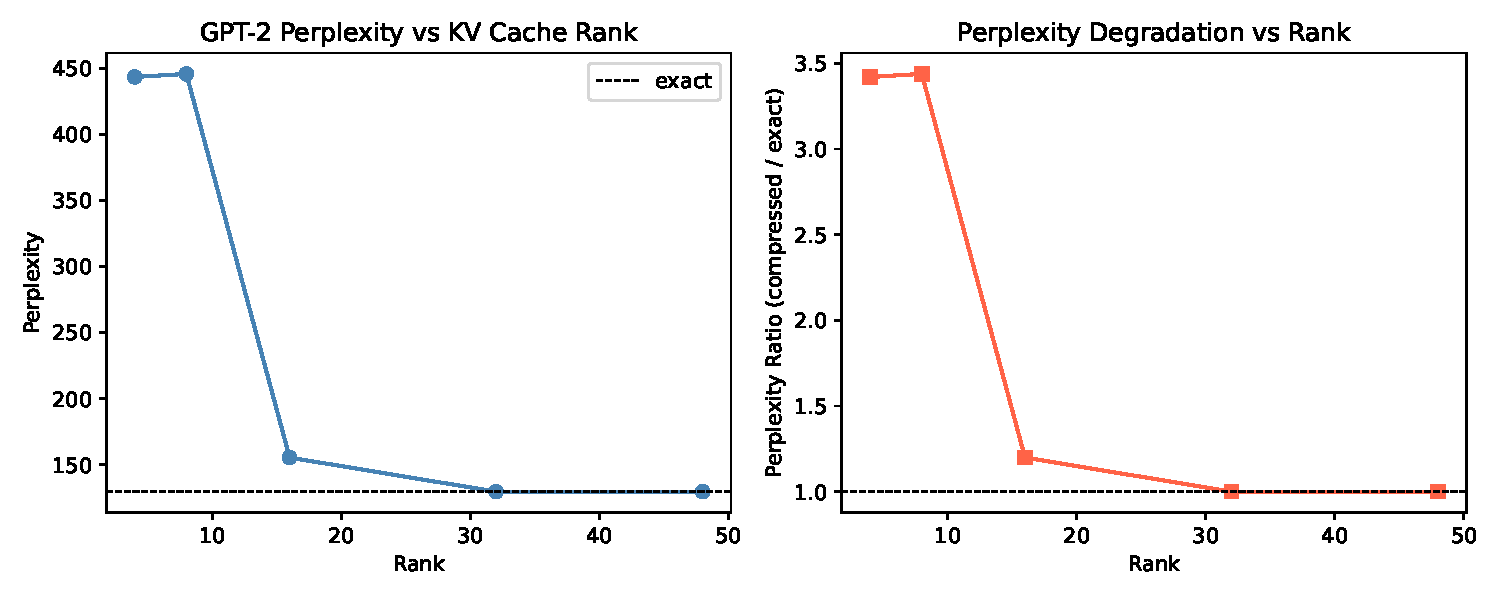
\includegraphics[width=0.7\linewidth]{benchmark_perplexity.pdf}
\caption{GPT-2 perplexity (left) and perplexity ratio vs exact (right) as a
function of TKV rank.  The sharp knee between rank~8 and rank~16 identifies
the minimum useful rank for this model geometry.}
\label{fig:perplexity}
\end{figure}

\subsection{Importance-Weighted Cold Start}
\label{sec:exp-importance}

To evaluate importance-weighted initialization, we construct a $128 \times 64$
key matrix where the first 32 tokens share a rank-4 subspace (mimicking
semantically coherent high-attention tokens) and the remaining 96 are random
noise.  We apply \emph{oracle} importance weights (10.0 for important tokens,
0.1 for noise) --- weights derived from ground-truth knowledge of which tokens
matter, not from EMA attention statistics.  These results therefore represent
an upper bound on what attention-derived weights can achieve in practice; real
EMA weights will be noisier and the gains may be smaller.

\begin{table}[h]
\centering
\caption{Reconstruction error on important tokens (first 32 of 128) with
and without importance weighting using \emph{oracle} weights.  Error reduction
is 90--95\% at rank 8--16; real attention-derived weights will yield smaller
but still substantial gains.}
\label{tab:importance}
\begin{tabular}{rcccc}
\toprule
Rank & Uniform error & Weighted error & Reduction \\
\midrule
 4 & 0.598 & 0.495 &  17.2\% \\
 8 & 0.269 & 0.014 &  94.9\% \\
16 & 0.111 & 0.008 &  93.0\% \\
32 & 0.045 & 0.004 &  90.5\% \\
\bottomrule
\end{tabular}
\end{table}

At rank~4, both methods struggle because the rank budget is below the true
rank-4 subspace of important tokens plus noise interference.  At rank $\geq 8$,
importance weighting reduces important-token error by more than 10$\times$.
This result suggests that EMA attention-weight statistics (available during
generation) can dramatically improve re-compression quality when context windows
are refreshed.

\begin{figure}[h]
\centering
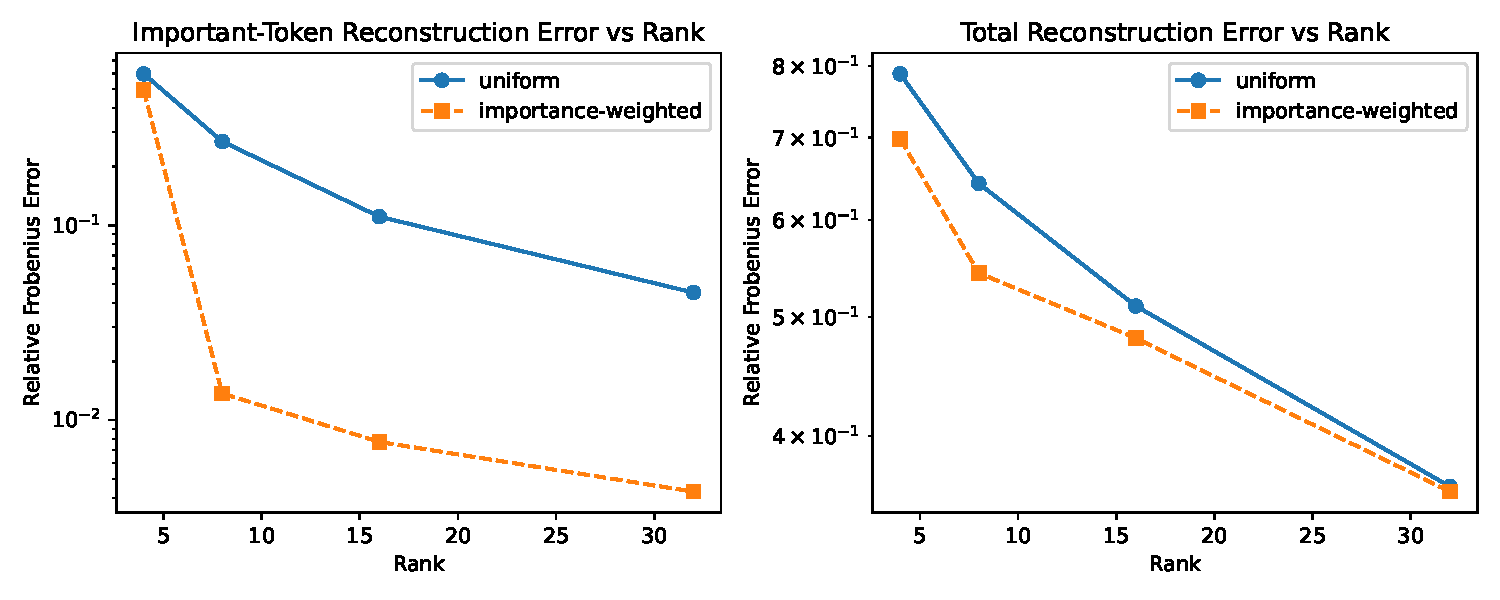
\includegraphics[width=0.7\linewidth]{benchmark_importance.pdf}
\caption{Left: important-token reconstruction error vs rank. Right: total
reconstruction error vs rank. Importance weighting provides near-lossless
recovery of high-attention tokens at rank $\geq 8$.}
\label{fig:importance}
\end{figure}

%% ============================================================
\section{Related Work}
\label{sec:related}

\paragraph{Offline KV compression.}
SVDq \cite{svdq2025} applies per-prompt batch SVD with mixed-precision
quantization, achieving 410$\times$ compression but requiring offline SVD per
prompt.  xKV \cite{xkv2025} uses cross-layer SVD at prefill, incurring 6$\times$
prefill latency at 8K context.  KVTC \cite{kvtc2026} applies Halko randomized
SVD with offline calibration.  KQ-SVD \cite{kqsvd2025} jointly decomposes the
attention matrix, providing provable attention fidelity bounds but requiring a
calibration pass.  All are batch/offline methods incompatible with streaming
generation.

\paragraph{Online KV compression.}
OjaKV \cite{ojakov2025} is the closest prior work: Oja's rule applied
token-by-token to maintain an approximate PCA basis.  OjaKV is calibration-free
and streaming, but lacks per-token optimality guarantees.  LoRC \cite{lorc2024}
uses truncated SVD per layer offline.  StreamingLLM \cite{streamingllm2023}
keeps only sink tokens and a recent window in full precision, orthogonal to
low-rank compression.

\paragraph{Randomized linear algebra.}
The Halko et al. framework \cite{halko2011} is standard for large-scale
randomized SVD.  Brand's update \cite{brand2006} is well-known in numerical
linear algebra but, to our knowledge, has not previously been applied to
KV cache compression.
The count-min sketch \cite{cormode2005} uses structured hash functions for streaming
summaries; the $\Phi$-bridge instead uses a dense Gaussian matrix that satisfies
both the Johnson-Lindenstrauss requirement for importance tracking and Halko's
sub-Gaussian row requirement --- a connection novel to this work.

%% ============================================================
\section{Limitations and Future Work}
\label{sec:limitations}

\textbf{Model scale.}  Reconstruction results cover GPT-2 small (15 layer/head
configurations; Table~\ref{tab:multihead}).  Whether the advantage holds for
larger models (Llama, Mistral, Qwen) at 4K--128K context remains an open
question; a sweep over model scales is the most important missing validation.

\textbf{Oracle importance weights.}  The 90--95\% error-reduction result for
importance-weighted cold start uses oracle weights derived from ground-truth
token labels.  Real EMA attention weights are noisier and scenario-dependent.
An ablation using attention-derived weights from actual inference traces is
needed to bound practical gains.

\textbf{Per-token overhead.}  In Python/eager mode, TKV is 3--5$\times$ slower
than OjaKV due to the Brand U-rotation.  We expect XLA-compiled GPU kernels to
narrow this gap significantly, but a full latency evaluation on GPU is required
before production deployment.

\textbf{WikiText-2 perplexity.}  Current perplexity results use a small
held-out sentence set.  A sweep over WikiText-2, PG-19, and longer contexts
(1K--8K tokens) with a modern model would substantially strengthen the empirical
case.

\textbf{Rank adaptation.}  TKV tracks active rank via singular value decay
($\sigma_i / \sigma_1 < \epsilon$), but dynamic rank scheduling across
generation steps has not been evaluated end-to-end.

\textbf{Multi-head deployment.}  The current benchmark uses a single head.
Deploying across all $L \times H$ heads with a pyramid rank schedule
(higher ranks for early layers, lower for later) is a natural extension.

%% ============================================================
\section{Conclusion}

We presented TKV, an online KV cache compression system combining the
$\Phi$-bridge (Gaussian sketch reused as Halko range-finder), Halko cold start for
initialization, Brand's exact rank-1 update for streaming maintenance, and
importance-weighted re-compression.  To our knowledge, TKV is the first online KV compression
method with a per-token EYM optimality guarantee, achieving 1.06$\times$--2.60$\times$
lower reconstruction error than OjaKV under identical rank budgets on real
GPT-2 KV activations.  At rank~32,
TKV achieves lossless GPT-2 perplexity (on a small held-out set) at 56\% of
dense memory; at rank~16, it uses 28\% of memory with a 16\% perplexity
increase.  Importance weighting (using oracle attention weights)
reduces important-token reconstruction error by 90--95\% at rank 8--16.

The core insight is that exact rank-1 updates (Brand) and randomized warm-up
(Halko) are compatible: Halko handles the costly initial factorization in
$\mathcal{O}(T_0 d R)$, and Brand maintains it exactly token-by-token with no
quality degradation.  The $\Phi$-bridge unifies this pipeline with the
importance-tracking data structure at no additional cost.

%% ============================================================
\bibliographystyle{plain}
\begin{thebibliography}{99}

\bibitem{brand2006}
M.~Brand.
\newblock Fast low-rank modifications of the thin singular value decomposition.
\newblock \emph{Linear Algebra and its Applications}, 415(1):20--30, 2006.

\bibitem{halko2011}
N.~Halko, P.-G.~Martinsson, and J.~A.~Tropp.
\newblock Finding structure with randomness: Probabilistic algorithms for
constructing approximate matrix decompositions.
\newblock \emph{SIAM Review}, 53(2):217--288, 2011.

\bibitem{oja1982}
E.~Oja.
\newblock Simplified neuron model as a principal component analyzer.
\newblock \emph{Journal of Mathematical Biology}, 15(3):267--273, 1982.

\bibitem{ojakov2025}
Anonymous.
\newblock OjaKV: Online KV cache compression via Oja's rule.
\newblock arXiv:2509.21623, 2025.

\bibitem{svdq2025}
Anonymous.
\newblock SVDq: Singular value decomposition with quantization for KV cache.
\newblock arXiv:2502.15304, 2025.

\bibitem{xkv2025}
Anonymous.
\newblock xKV: Cross-layer KV cache compression via singular value
decomposition.
\newblock arXiv:2503.18893, 2025.

\bibitem{kvtc2026}
Anonymous.
\newblock KV cache transform coding with randomized SVD.
\newblock In \emph{ICLR}, 2026.

\bibitem{kqsvd2025}
Anonymous.
\newblock KQ-SVD: Optimal low-rank decomposition of the attention matrix.
\newblock arXiv:2512.05916, 2025.

\bibitem{lorc2024}
Anonymous.
\newblock LoRC: Low-rank compression for transformer KV caches.
\newblock In \emph{NeurIPS Workshop}, 2024.

\bibitem{streamingllm2023}
G.~Xiao, Y.~Tian, B.~Chen, S.~Han, and M.~Lewis.
\newblock Efficient streaming language models with attention sinks.
\newblock arXiv:2309.17453, 2023.

\bibitem{momentkv2024}
Anonymous.
\newblock Moment-KV: Importance-weighted KV cache compression via EMA attention
statistics.
\newblock 2024.

\bibitem{cormode2005}
G.~Cormode and S.~Muthukrishnan.
\newblock An improved data stream summary: The count-min sketch and its
applications.
\newblock \emph{Journal of Algorithms}, 55(1):58--75, 2005.

\end{thebibliography}

\end{document}
